\documentclass[a4paper, 12pt]{article}

\usepackage{amsmath}
\usepackage{amssymb}
\usepackage{graphicx}
\usepackage{listings}[language=C++]
\lstdefinestyle{mystyle}{
    breakatwhitespace=false,         
    breaklines=true,                 
    captionpos=b,                    
    keepspaces=true,                 
    numbers=left,                    
    numbersep=5pt,                  
    showspaces=false,                
    showstringspaces=false,
    showtabs=false,                  
    tabsize=2
}

\lstset{style=mystyle}

\title{Lab-07 Report}
\author{st122246}

\begin{document}
	\maketitle

	\section{PySLAM on Video Datatset}
	
	\begin{figure}
		\caption{Video Dataset}
		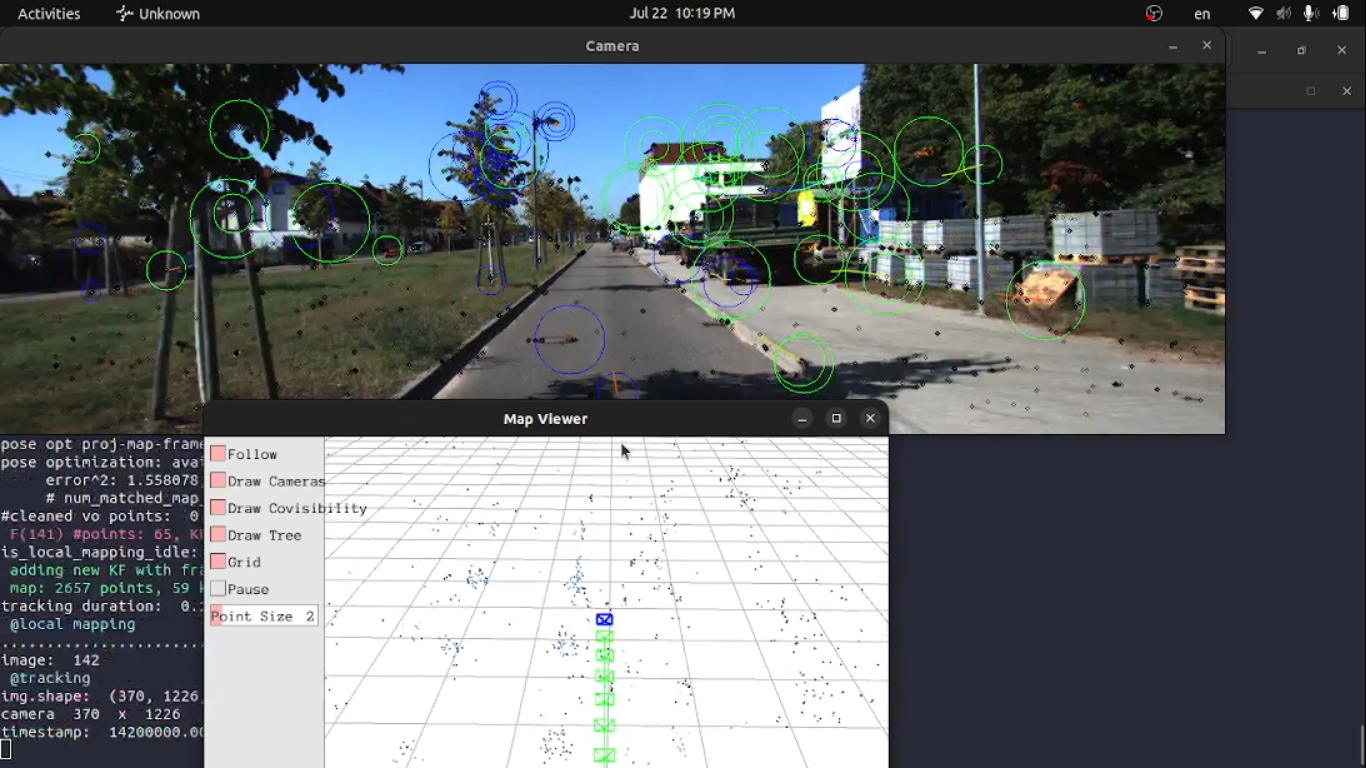
\includegraphics[scale=0.25]{images/video.png}
	\end{figure}

\section{PySLAM on TUM Dataset}

	\begin{lstlisting}
//config.ini
[DATASET]
; select your dataset (decomment only one of the following lines!) 
;type=KITTI_DATASET
type=TUM_DATASET
;type=VIDEO_DATASET
;type=FOLDER_DATASET
;type=LIVE_DATASET
;type=RC_DATASET
	\end{lstlisting}
	
	\begin{figure}
		\caption{TUM Dataset}
		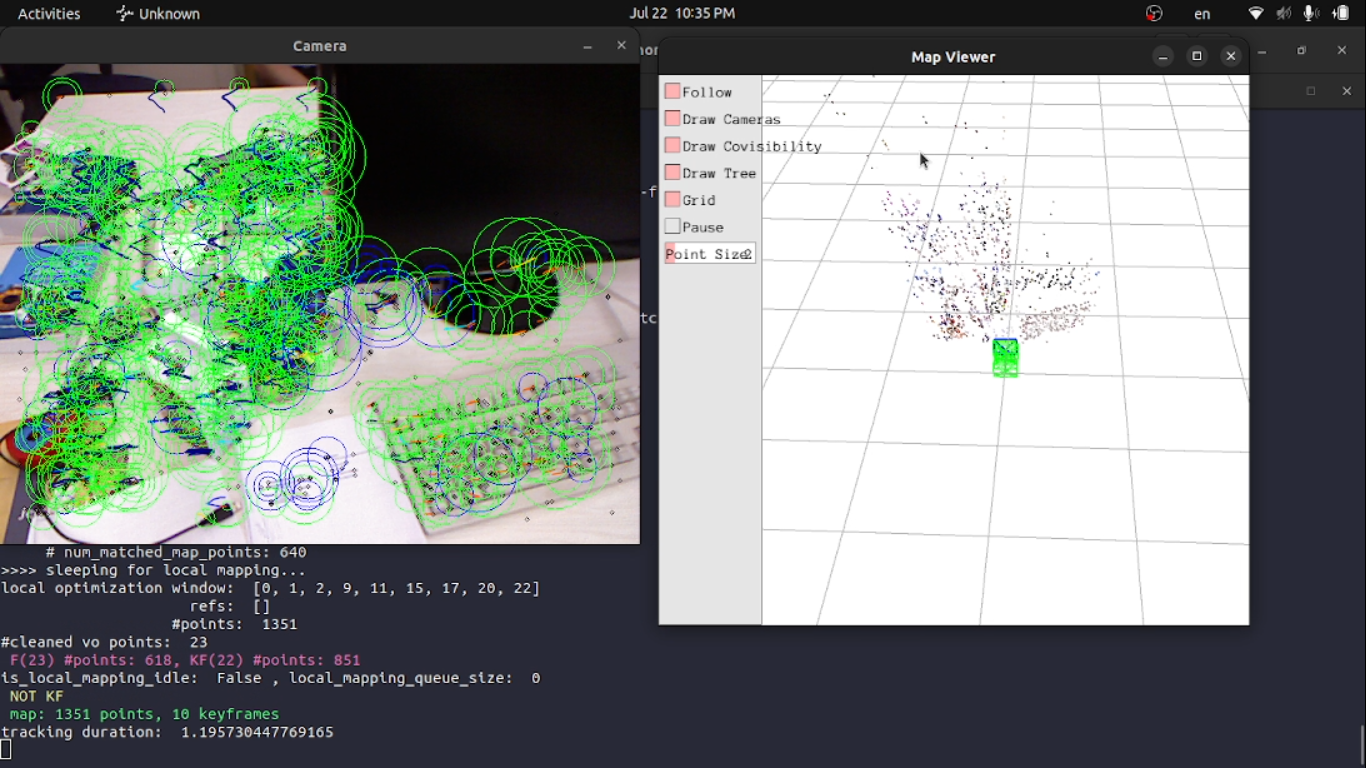
\includegraphics[scale=0.25]{images/TUM.png}
	\end{figure}

	\section{PySLAM on Own Video}

	\begin{lstlisting}
//config.ini
[DATASET]
; select your dataset (decomment only one of the following lines!) 
;type=KITTI_DATASET
;type=TUM_DATASET
;type=VIDEO_DATASET
;type=FOLDER_DATASET
;type=LIVE_DATASET
type=RC_DATASET

[RC_DATASET]
type=video
base_path=/mnt/ntfs/Data/code/CV/computer_vision/Labs/Data/Lab07/rc_car
cam_settings=settings/rc_car.yaml
name=car.mp4
groundtruth_file=auto
	\end{lstlisting}

	\begin{lstlisting}
//rc_car.yaml
#--------------------------------------------------------------------------------------------
# Viewer Parameters
#--------------------------------------------------------------------------------------------
# Viewer.on: 1 is ON, 0 is OFF
Viewer.on: 1

Viewer.KeyFrameSize: 0.05
Viewer.KeyFrameLineWidth: 1
Viewer.GraphLineWidth: 0.9
Viewer.PointSize: 1
Viewer.LineSize: 1
Viewer.CameraSize: 0.08
Viewer.CameraLineWidth: 3
Viewer.ViewpointX: 0
Viewer.ViewpointY: -0.7
Viewer.ViewpointZ: -1.8
Viewer.ViewpointF: 500

#--------------------------------------------------------------------------------------------
# Camera Parameters. Adjust them!
#--------------------------------------------------------------------------------------------

#camera matrix:
# [[544.06254343   0.         321.767787]
# [  0.         548.01458 271.29350075]
# [  0.           0.           1.        ]]
#distortion coefficients:  [0.14004592 -0.61955377 0.02033056  0.01136857 0.45179258]


# Camera calibration and distortion parameters (OpenCV) 
Camera.fx: 544.06254343
Camera.fy: 548.01458
Camera.cx: 321.767787
Camera.cy: 271.29350075

Camera.k1: 0.14004592
Camera.k2: -0.61955377
Camera.p1: 0.02033056
Camera.p2: 0.01136857
Camera.k3: 0.45179258

Camera.width: 640
Camera.height: 480

# Camera frames per second 
Camera.fps: 30.0

# IR projector baseline times fx (aprox.)
Camera.bf: 40.0

# Color order of the images (0: BGR, 1: RGB. It is ignored if images are grayscale)
Camera.RGB: 0

# Close/Far threshold. Baseline times.
ThDepth: 40.0

# Deptmap values factor
DepthMapFactor: 1.0

#--------------------------------------------------------------------------------------------
# ORB Parameters
#--------------------------------------------------------------------------------------------

# ORB Extractor: Number of features per image
ORBextractor.nFeatures: 1000

# ORB Extractor: Scale factor between levels in the scale pyramid 	
ORBextractor.scaleFactor: 1.2

# ORB Extractor: Number of levels in the scale pyramid	
ORBextractor.nLevels: 8

# ORB Extractor: Fast threshold
# Image is divided in a grid. At each cell FAST are extracted imposing a minimum response.
# Firstly we impose iniThFAST. If no corners are detected we impose a lower value minThFAST
# You can lower these values if your images have low contrast			
ORBextractor.iniThFAST: 20
ORBextractor.minThFAST: 7
	\end{lstlisting}
	
	\begin{figure}
		\caption{Own Video}
		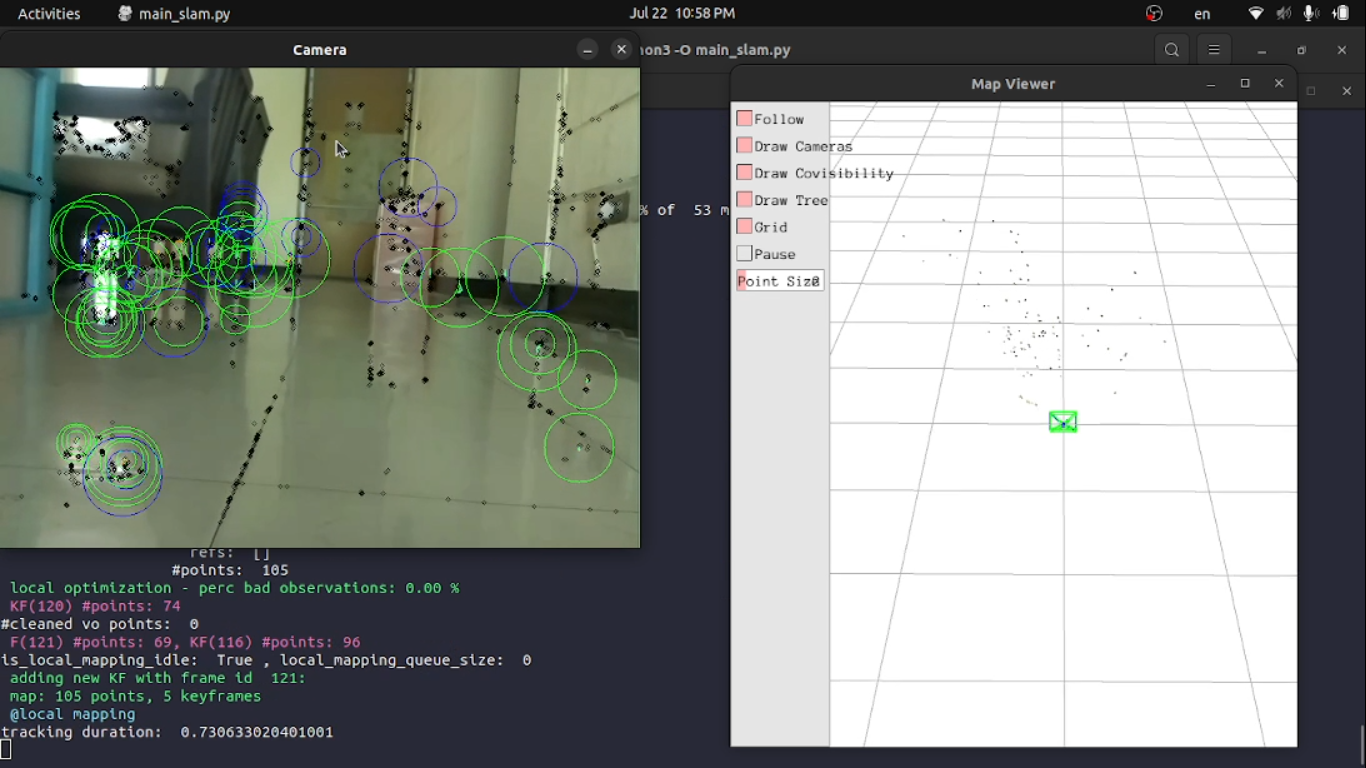
\includegraphics[scale=0.25]{images/own.png}
	\end{figure}
\end{document}